% Chapter 3: Theory Development
\chapter{Theory Development}
\label{chapter:theory-development}

\graphicspath{ {report/C3 Theory Development/assets/} } 

\section{Theoretical Development of SSVEP Decoding Algorithms}

\subsection{Canonical correlation analysis (CCA)}
\label{section:cca-c3}
Given variable partitions $\mX \in \R^{m\times p}$, $\mY \in \R^{m\times q}$ each with $m$ observations, CCA seeks to find a linear combination of $\mX$, $\mY$ that maximises the correlation between their images. More formally, assuming that the variables (columns) of the two partitions $\vx_1, \dots, \vx_p \in \R^{m}$ and $\vy_1, \dots, \vy_q \in \R^{m}$ are standardised to have zero mean and unit variance, find
\begin{align}
    \rho &= \max_{\vw_X, \vw_Y} \textrm{corr}(\mX \vw_X, \mY \vw_Y) \\
    &= \max_{\vw_X, \vw_Y} \frac{\E[\mX \vw_X\vw_Y^\top\mY^\top ]}{\sqrt{\E[\mX \vw_X\vw_X^\top\mX^\top]\E[\mY \vw_Y\vw_Y^\top\mY^\top]}}
    \label{eq:cca-corr-objective}
\end{align}
where $\rho$ is the \textit{canonical correlation}, $\vw_X$ and $\vw_Y$ are the canonical weight vectors and the images $\vz_X = \mX\vw_X$ and $\vz_Y = \mY\vw_Y$ are the \textit{canonical variables} for $\mX$ and $\mY$ respectively.

\subsubsection{Geometric interpretation}
The authors in \cite{cca-tutorial} present an intuitive geometric analogy. Consider $\mX$ and $\mY$ as linear transforms of position vectors $\vw_X$ and $\vw_Y$ onto their images $\vz_X$ and $\vz_Y$ in $\R^m$. CCA constrains $\vz_X$ and $\vz_Y$ to have unit norm and that the angle $\theta \in [0, \frac{\pi}{2}]$ between them be minimised so as to maximise their correlation. The canonical correlation $\rho$ is then the inner product of $\vz_X$ and $\vz_Y$:
\begin{equation}
    \rho = \vz_X^\top\vz_Y = \|\vz_X\| \|\vz_Y\|\cos(\theta) = \cos(\theta)
\end{equation}
Therefore, CCA aims to find position vectors $\vw_X$, $\vw_Y$ that, after undergoing linear transforms $\mX$ and $\mY$, are mapped to a unit sphere in $\R^m$ where $\theta$ is minimised \cite{cca-tutorial}. Note that there will be $n=\textrm{min}(p, q)$ canonical correlations $\rho_1, \dots, \rho_n$ with $|\rho_i| \geq |\rho_j|, \; \forall \; i < j$. Typically, only the first and largest canonical correlation $\rho_1$ is considered. 

\subsubsection{Solving for canonical weight vectors through the eigenvalue problem}
Consider the case of solving for the first and largest canonical correlation $p_1$. Following the geometric interpretation, the objective is to find
\begin{equation}
    \cos(\theta_1) = \max_{\vw_X, \vw_Y}\langle\,\vz_X,\vz_Y\rangle \quad \textrm{with} \quad \|\vz_X\| = \|\vz_Y\| = 1
\label{eq:cca-objective-1}
\end{equation}
where $\theta_1$ is the smallest angle between image vectors. Defining the within-set covariance matrices as 
\begin{align}
    \mC_{XX} = \mX^\top\mX \quad \textrm{and} \quad
    \mC_{YY} = \mY^\top \mY 
\end{align}
and the inter set cross covariance matrix as 
\begin{align}
    \mC_{XY} &= \mX^\top\mY,
\end{align}
the unit variance constraint on the image vectors can be rewritten as  \begin{align}
\begin{split}
    \|\vz_X\| &= \vz_X^\top\vz_X = \vw_X^\top \mX^\top \mX \vw_X =  \vw_X^\top \mC_{XX} \vw_X = 1 \\
    \|\vz_Y\| &= \vz_Y^\top\vz_Y = \vw_Y^\top \mY^\top \mY \vw_Y =  \vw_Y^\top \mC_{YY} \vw_Y = 1 
    \end{split}
\label{eq:unit-variance-reformulated}
\end{align}
Substituting (\ref{eq:unit-variance-reformulated}) into (\ref{eq:cca-corr-objective}) yields 

\begin{equation}
\cos(\theta) = \max_{\vw_X, \vw_Y} \vw_X^\top \mC_{XY} \vw_Y 
\end{equation}
Lagrangian dual theory provides a straight forward way to solve the constrained optimisation problem above with unit variance constraints as in (\ref{eq:unit-variance-reformulated}). Consider the Lagrangian for this problem below with Lagrange multipliers $\lamba_1$ and $\lambda_2$:
\begin{equation}
    \mathcal{L}(\vw_X, \vw_Y, \lambda_1, \lambda_2) = \vw_X^\top \mC_{XY} \vw_Y - \frac{\lambda_1}{2}(\vw_X^\top \mC_{XX} \vw_X-1) - \frac{\lambda_2}{2}(\vw_Y^\top \mC_{YY} \vw_Y-1)
\end{equation}
With reference to the KKT conditions, stationary requires
\begin{align}
    \label{eq:cca-lagrange-x}
    \frac{\partial \mathcal{L}}{\partial \vw_X} &= \mC_{XY} \vw_Y - \lambda_1\mC_{XX} \vw_X = 0 \\
    \frac{\partial \mathcal{L}}{\partial \vw_Y} &= \mC_{YX} \vw_X - \lambda_2\mC_{YY} \vw_Y = 0
        \label{eq:cca-lagrange-y}
\end{align}
Since $\mC_{YX} = \mC_{XY}^\top$. Pre-multiplying (\ref{eq:cca-lagrange-x}) by $\vw_X^\top$ and (\ref{eq:cca-lagrange-y}) by $\vw_Y^\top$ yields:
\begin{align}
\begin{split}
    \vw_X^\top\mC_{XY} \vw_Y - \lambda_1\vw_X^\top\mC_{XX} \vw_X &= 0 \\
    \vw_Y^\top\mC_{YX} \vw_X - \lambda_2\vw_Y^\top\mC_{YY} \vw_Y &= 0
\end{split}
\label{eq:lagrange-multi}
\end{align}
Since $\vw_X^\top \mC_{XX} \vw_X = \vw_Y^\top \mC_{YY} \vw_Y =1$, it is clear from (\ref{eq:lagrange-multi}) that $\lambda_1=\lambda_2 = \lambda$. Substituting this result into (\ref{eq:cca-lagrange-x}) yields
\begin{align}
    \vw_X = \frac{\mC_{XX}^{-1}C_{XY}\vw_Y}{\lambda}
\end{align}
Then, substituting into (\ref{eq:cca-lagrange-y}) produces the following generalised eigenvalue problem:
\begin{align}
    \mC_{YX}\mC^{-1}_{XX}\mC_{XY}\vw_{Y} = \lambda^2\mC_{YY}\vw_Y
\end{align}
If $\mC_{YY}$ is non-singular, this reduces to a standard eigenvalue problem of the form
\begin{align}
    \mC_{YY}^{-1}\mC_{YX}\mC^{-1}_{XX}\mC_{XY}\vw_{Y} = \lambda^2\vw_Y
\end{align}
The eigenvalues of the matrix $\mC_{YY}^{-1}\mC_{YX}\mC^{-1}_{XX}\mC_{XY}$ correspond to the squares of the canonical correlations $\rho_1, \dots, \rho_n$.

\subsection{Multiset CCA (MsetCCA)}
MsetCCA is an extension of standard CCA to multiple data sets or partitions. Accordingly, the objective is now to maximise the correlation between canonical variables from \textit{many sets} of observations at a given stimulus frequency $f_k$. MsetCCA extends the signal matrix $\mX\in \R^{N_s \times N_c}$ to a third order signal tensor $\tX \in \R^{N_s \times N_c \times N_t}$ with $N_t$ trials, each with $N_c$ channels\footnote{the constraint that the number of variables (width of $\mX_i$) for each trial be constant is not strictly necessary. For this application, however, it is assumed that the number of channels will not change between trials of a given experiment.} and $N_s$ samples. Although several objective functions for MsetCCA exist, the MAXVAR objective is explored in \cite{zhang-mset-cca} for its intuitive extension to ordinary CCA with multiple variable sets. Assuming all sets of variables in $\tX$ are normalised to have zero mean and unit variance, the MAXVAR objective for maximising correlation over canonical variables from multiple sets at a given candidate frequency $f_k$ is defined as follows:
\begin{align}
\begin{split}
\max_{\mathbf{w}_{1}, \ldots, \mathbf{w}_{N_t}} & \quad \rho=\sum_{i \neq j}^{N_t} \mathbf{w}_{i}^\top\mX_{i}^\top \mX_{j}\mathbf{w}_{j} \\
\text { s.t. } & \quad \frac{1}{N_t} \sum_{i=1}^{N_t} \mathbf{w}_{i}^\top\mX_{i}^\top \mX_{i}\mathbf{w}_{i}=1
\end{split}
\label{eq:mset-cca-objective}
\end{align}
Following a similar approach as in the derivation for CCA above, the method of Lagrange multipliers can be used to transform the constrained optimisation problem in (\ref{eq:mset-cca-objective}) to a generalised eigenvalue problem of the form:
\begin{equation}
        (\mR -\mS)\vw = \rho\mS \vw
\label{eq:mset-cca-gen-eig}
\end{equation}
where
\begin{align*}
\mR = \begin{bmatrix}
\mX_{1}^{\top}\mX_{1} & \ldots & \mX_{1}^{\top}\mX_{N_t} \\
\vdots & \ddots & \vdots \\
\mX_{N_t}^{\top}\mX_{1} & \ldots & \mX_{N_t}^{\top} \mX_{N_t}
\end{bmatrix},
\quad
\mS = \begin{bmatrix}
\mX_{1}^{\top}\mX_{1} & \ldots & 0 \\
\vdots & \ddots & \vdots \\
0 & \ldots & \mX_{N_t}^{\top} \mX_{N_t}
\end{bmatrix}
\quad
\textrm{and}
\quad
\vw = \begin{bmatrix}
\vw_1 \\ \vdots \\ \vw_{N_t}
\end{bmatrix}
\end{align*}
Thus, $\mR$ is the inter-trial block covariance matrix which captures sub-covariance matrices between all pairs of trials $n\in \{1, \dots, N_t \}$. $\mS$ is a block diagonal matrix which captures within-set covariance matrices for each trial. $\vw$ is a matrix of optimal spatial filters (vectors) $\vw_1, \dots, \vw_{N_t}$ resulting from the largest combined canonical correlation between all canonical variables $\vz_i = \mX_i\vw_i \in \R^{N_s}, \; \forall \; i\in[1, \; N_t]$. As with standard CCA, the largest canonical correlation $\rho^*$ corresponds to the largest generalised eigenvalue in (\ref{eq:mset-cca-gen-eig}). The canonical variables $\vz_i$ corresponding to $\rho^*$ are indeed the eigenvectors corresponding to the largest generalised eigenvalue \cite{zhang-mset-cca}. The optimal reference $\mY_k \in \R^{N_s \times N_t}$ for given frequency $f_k$ can be computed using the spatial filters from $\vw$ as:
\begin{align}
    \mY_k =
    \begin{bmatrix}
    \vz_{1, \, k} & \dots & \vz_{N_t, \,k}
    \end{bmatrix}
    =
    \begin{bmatrix}
    \mX_{1, \, k}\vw_{1, \, k}  & \dots & \mX_{N_t, \,k}\vw_{N_t,\, k} 
    \end{bmatrix}
\end{align}

After this training or calibration process is complete and $\mY_k$ is computed for all candidate frequencies $f_k$, these optimised reference sets can be used for inference. Given a new set of test signals $\hat{\mX} \in \R^{N_s \times N_c}$, ordinary CCA as in Section \ref{section:cca-c3} can be used to discern the frequency $f^$ corresponding to the highest canonical correlation between $\hat{\mX}$ and the associated referenced set $\mY^*$. The process for finding $f^*$ is identical to that in (\ref{eq:cca-freq-discrimination}). The important difference here is how the pre-computed reference sets $\mY_k$ used in the CCA algorithm are calculated.

\subsection{Generalised CCA (GCCA)}


\begin{figure}[h]
    \centering
    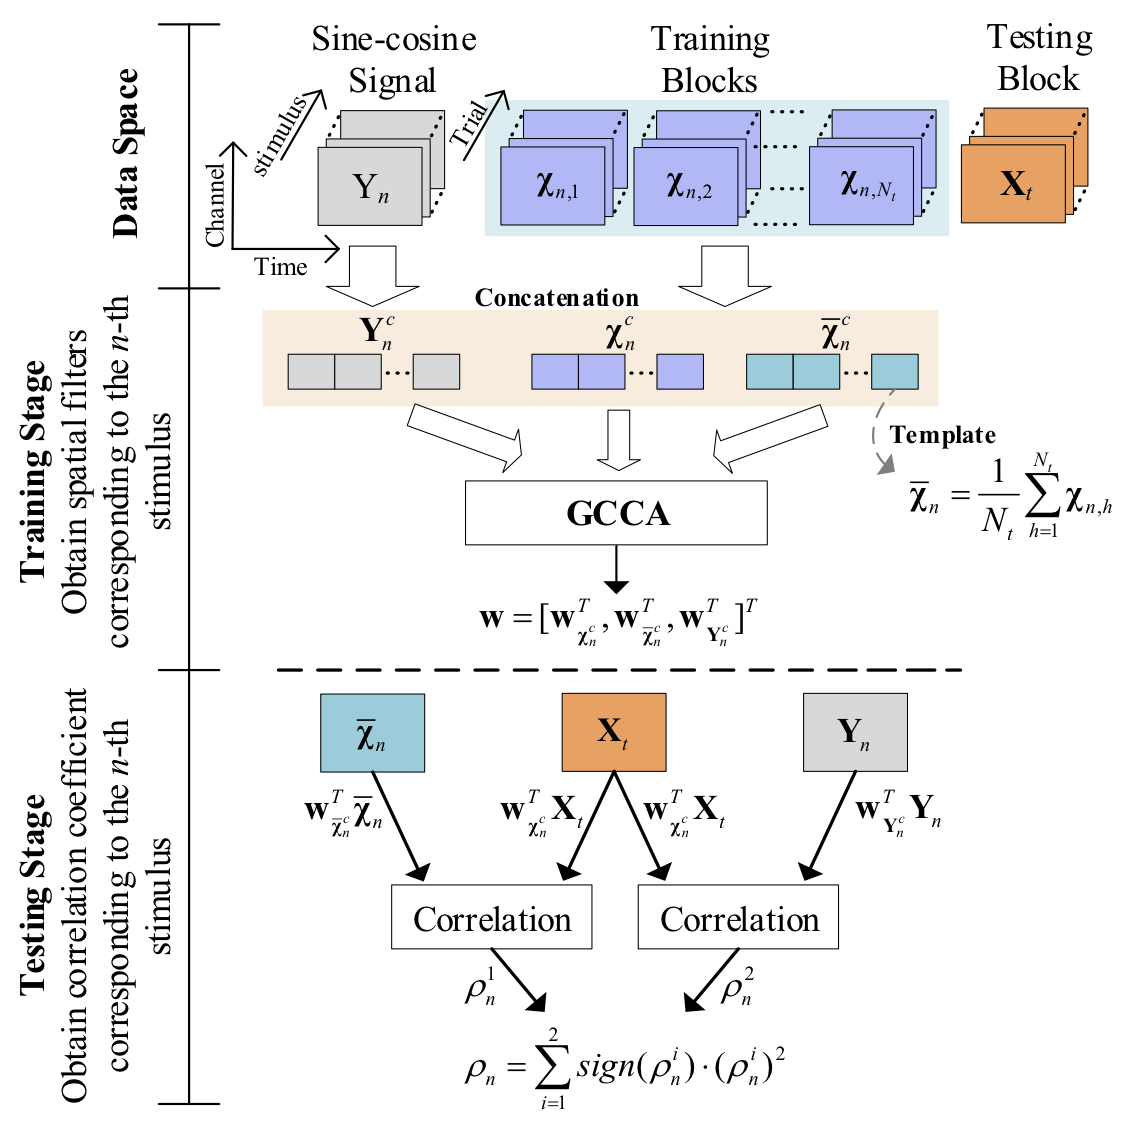
\includegraphics[width=0.55\textwidth]{gcca}
    \caption[Overview of the generalised CCA (GCCA) algorithm]{Diagram of the GCCA algorithm for SSVEP signal recognition. Extracted from \cite{sun-gcca}.}
    \label{fig:gcca}
\end{figure}

\subsection{Task-related component analysis (TRCA)}

\subsection{Related theory}
\subsubsection{Significance testing}
\subsubsection{Quantifying signal quality}
\subsubsection{Mechanics of sampling}